\documentclass{beamer}
\usepackage[utf8]{inputenc}

\usepackage{amsmath}
\usepackage{graphicx}
\usepackage{url}
\usepackage{fancyvrb}
\usepackage{xcolor}

\usetheme{Antibes}
\usecolortheme{whale}
\usepackage{lmodern}

\usepackage{listings}

\mode<presentation>

\definecolor{orange}{HTML}{BC2E07}

\usepackage{hyperref}
\hypersetup{
    colorlinks,
    linkcolor=orange,
    urlcolor=blue
}

\title{Lab \# 2: Introduction to Programming}
\subtitle{EC-102 -- Computer Systems and Programming}

\author{Usama Wajhi}
\institute{School of Mechanical and Manufacturing Engineering (SMME), \\ National University of Sciences and Technology (NUST)}
\date{\today}

\begin{document}
\begin{frame}
    \titlepage
\end{frame}

\begin{frame}
    \frametitle{Outline}
    \begin{columns}
        \column{0.5\textwidth}
        \tableofcontents
        \column{0.5\textwidth}
        \begin{figure}
            \centering
            
\includegraphics[scale=0.14]{programming}
        \end{figure}
    \end{columns}
\end{frame}

\begin{frame}
    \frametitle{Lab Grading Criteria}
    \section{Lab Grading} % (fold)
    \label{sec:lab_grading}
    \begin{itemize}
        \item Lab Work and Lab Report $\sim$ 50\%
        \begin{itemize}
            \item Lab work represents your performance in lab assignments/tasks. Every student will be graded individually.
            \item Lab report may be submitted by a group of max 5 students. Make sure that you submit one lab report per week.
        \end{itemize}
        \item Projects $\sim$ 40\%
        (details will be provided later)
        \item Attendance $\sim$ 10\%
    \end{itemize}
\end{frame}

\begin{frame}
    \frametitle{Lab Report: Contents}
    \section{Lab Report} % (fold)
    \label{sec:lab_report}
    \subsection{Lab Report Contents} % (fold)
    \label{sub:lab_report_contents}
    \begin{itemize}
        \item Problem statement
        \item Algorithm
        \item Flow chart
        \item Code
        \item Conclusion
    \end{itemize}
\end{frame}

\begin{frame}
    \frametitle{Lab Report: Title Page}
    \subsection{Lab Report Title} % (fold)
    \label{sub:lab_report_title}
    \begin{itemize}
        \item Name of school and university
        \item Name of subject
        \item Lab number and topic
        \item Submitted to
        \item Submitted by ( Name and Reg No)
        \item Date
    \end{itemize}
\end{frame}

\begin{frame}
    \frametitle{Basics of Computer Programming}
    \section{Basics of Computer Programming}
    \subsection{What is a computer system?} % (fold)

    \label{subsec:what_is_a_computer_system}
    A \textbf{computer system} is one that is able to take a set of inputs, process them and create a set of useful outputs.

    \begin{figure}
        \centering
        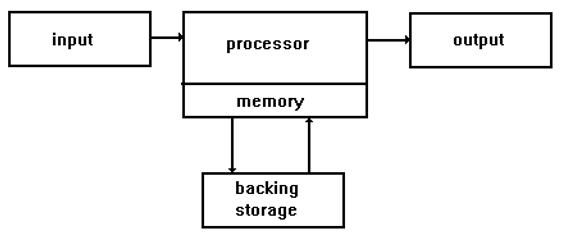
\includegraphics[scale=0.3]{comp_sys}
    \end{figure}

    \par
    One or more \emph{input}s are used to provide data, this data is then \emph{processed in some way} and the outcome of processing is sent to an \emph{output} or it may be stored until some event happens and brings it to the output. \\

    \subsection{What is a computer program?} % (fold)
    \label{subsec:what_is_a_computer_program}
    For processing to take place, there needs to be a set of instructions of what needs to be done. This set of instructions is known as a \textbf{computer program}.
\end{frame}

\begin{frame}
    \frametitle{Why Study Programming?}
    \subsection{Why study programming?} % (fold)
    \label{subsec:why_study_programming}
    \begin{itemize}
        \item Automation -- home, industrial
        \begin{columns}
            \column{0.5\textwidth}
            \begin{figure}
                \centering
                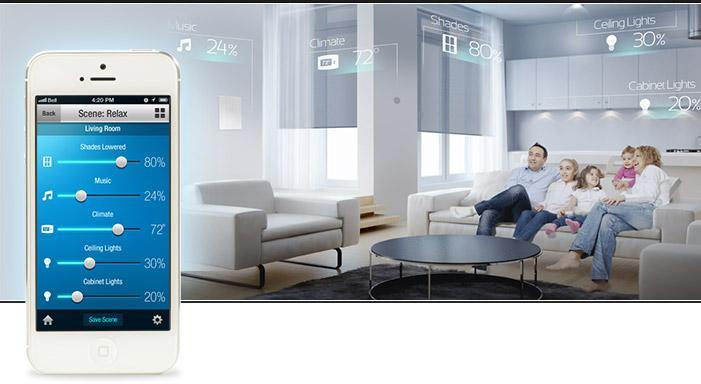
\includegraphics[scale=0.33]{home_automation}
            \end{figure}
            \column{0.5\textwidth}
            \begin{figure}
                \centering
                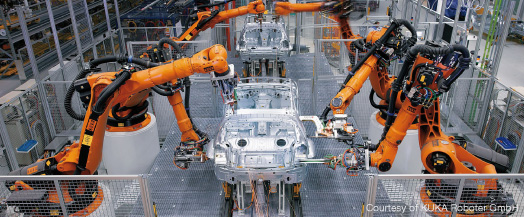
\includegraphics[scale=0.33]{industrial_automation}
            \end{figure}
        \end{columns}
    \end{itemize}
\end{frame}

\begin{frame}
    \frametitle{Why Study Programming?}
    \begin{itemize}
        \item Robotics -- wheeled, aerial, humanoid
        \begin{columns}
            \column{0.25\textwidth}
            \begin{figure}
                \centering
                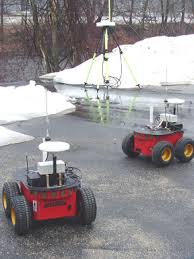
\includegraphics[scale=0.45]{wheeled}
            \end{figure}
            \column{0.35\textwidth}
            \begin{figure}
                \centering
                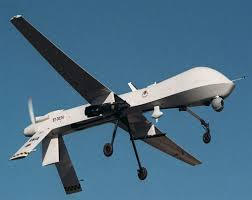
\includegraphics[scale=0.45]{aerial}
            \end{figure}
            \column{0.4\textwidth}
            \begin{figure}
                \centering
                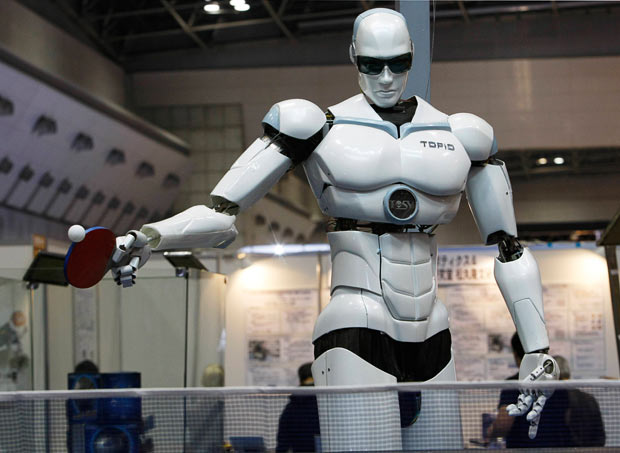
\includegraphics[scale=0.22]{humanoid}
            \end{figure}
        \end{columns}
    \end{itemize}
\end{frame}

\begin{frame}
    \frametitle{Why Study Programming?}
    \begin{itemize}
        \item Computer Vision -- face recognition, image filtering
        \begin{columns}
            \column{0.5\textwidth}
            \begin{figure}
                \centering
                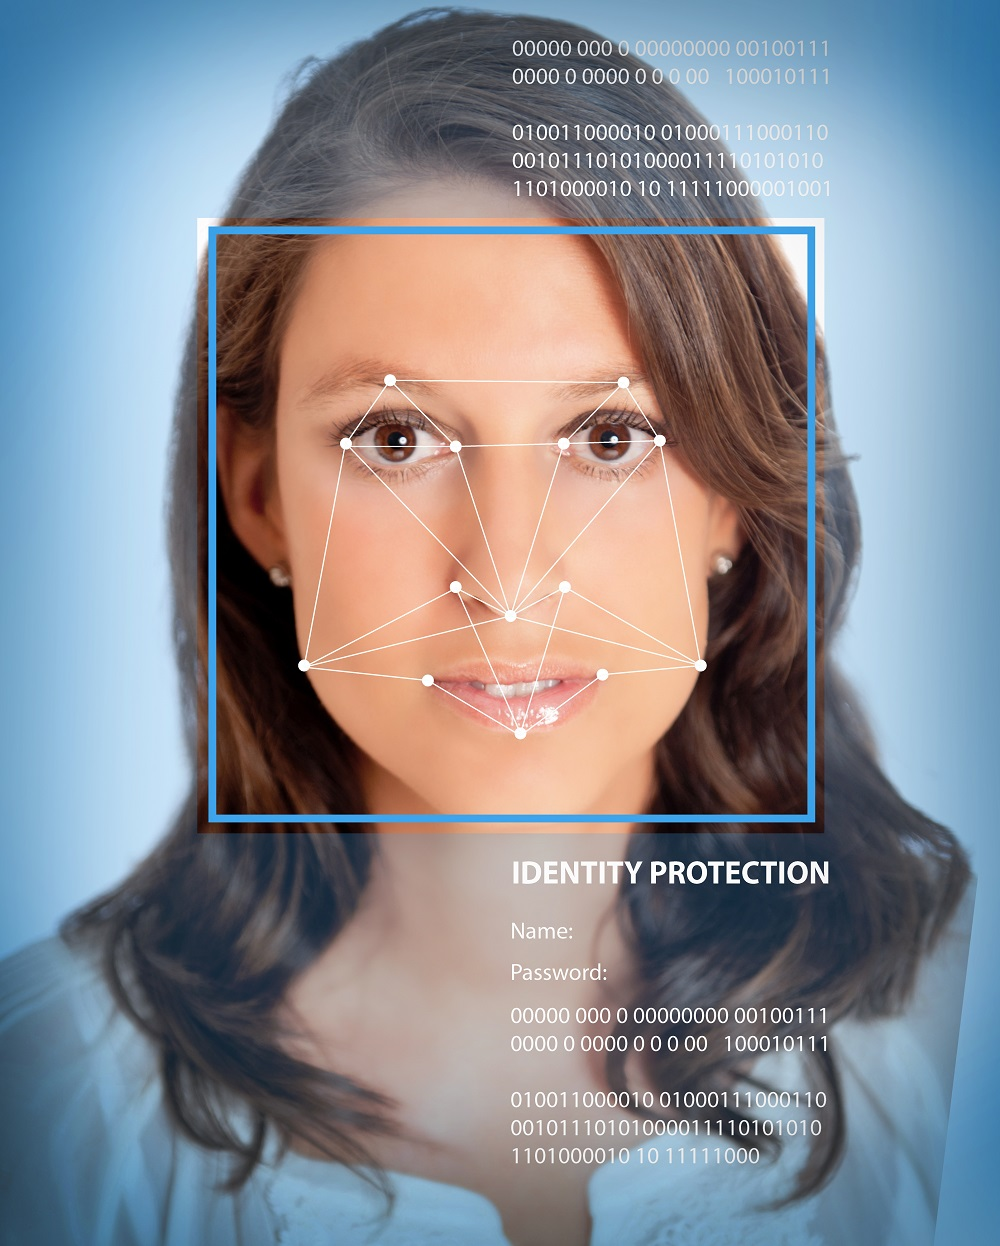
\includegraphics[scale=0.47]{face_recog}
            \end{figure}
            \column{0.5\textwidth}
            \begin{figure}
                \centering
                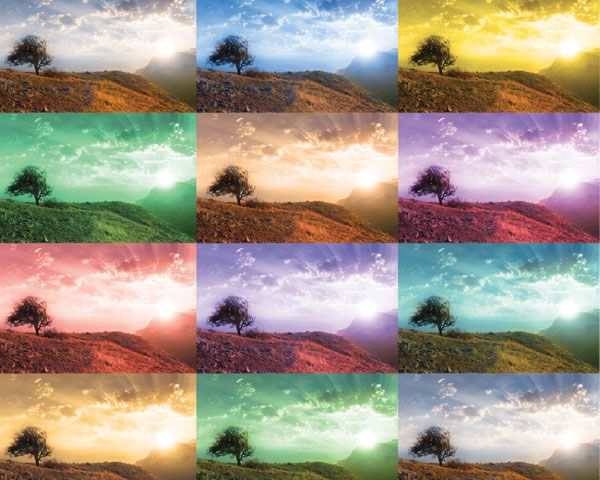
\includegraphics[scale=0.26]{filtering}
            \end{figure}
        \end{columns}
    \end{itemize}
\end{frame}

\begin{frame}
    \frametitle{Why Study Programming?}
    \begin{itemize}
        \item Movies -- computer generated imagery, motion capture
        \begin{columns}
            \column{0.5\textwidth}
            \begin{figure}
                \centering
                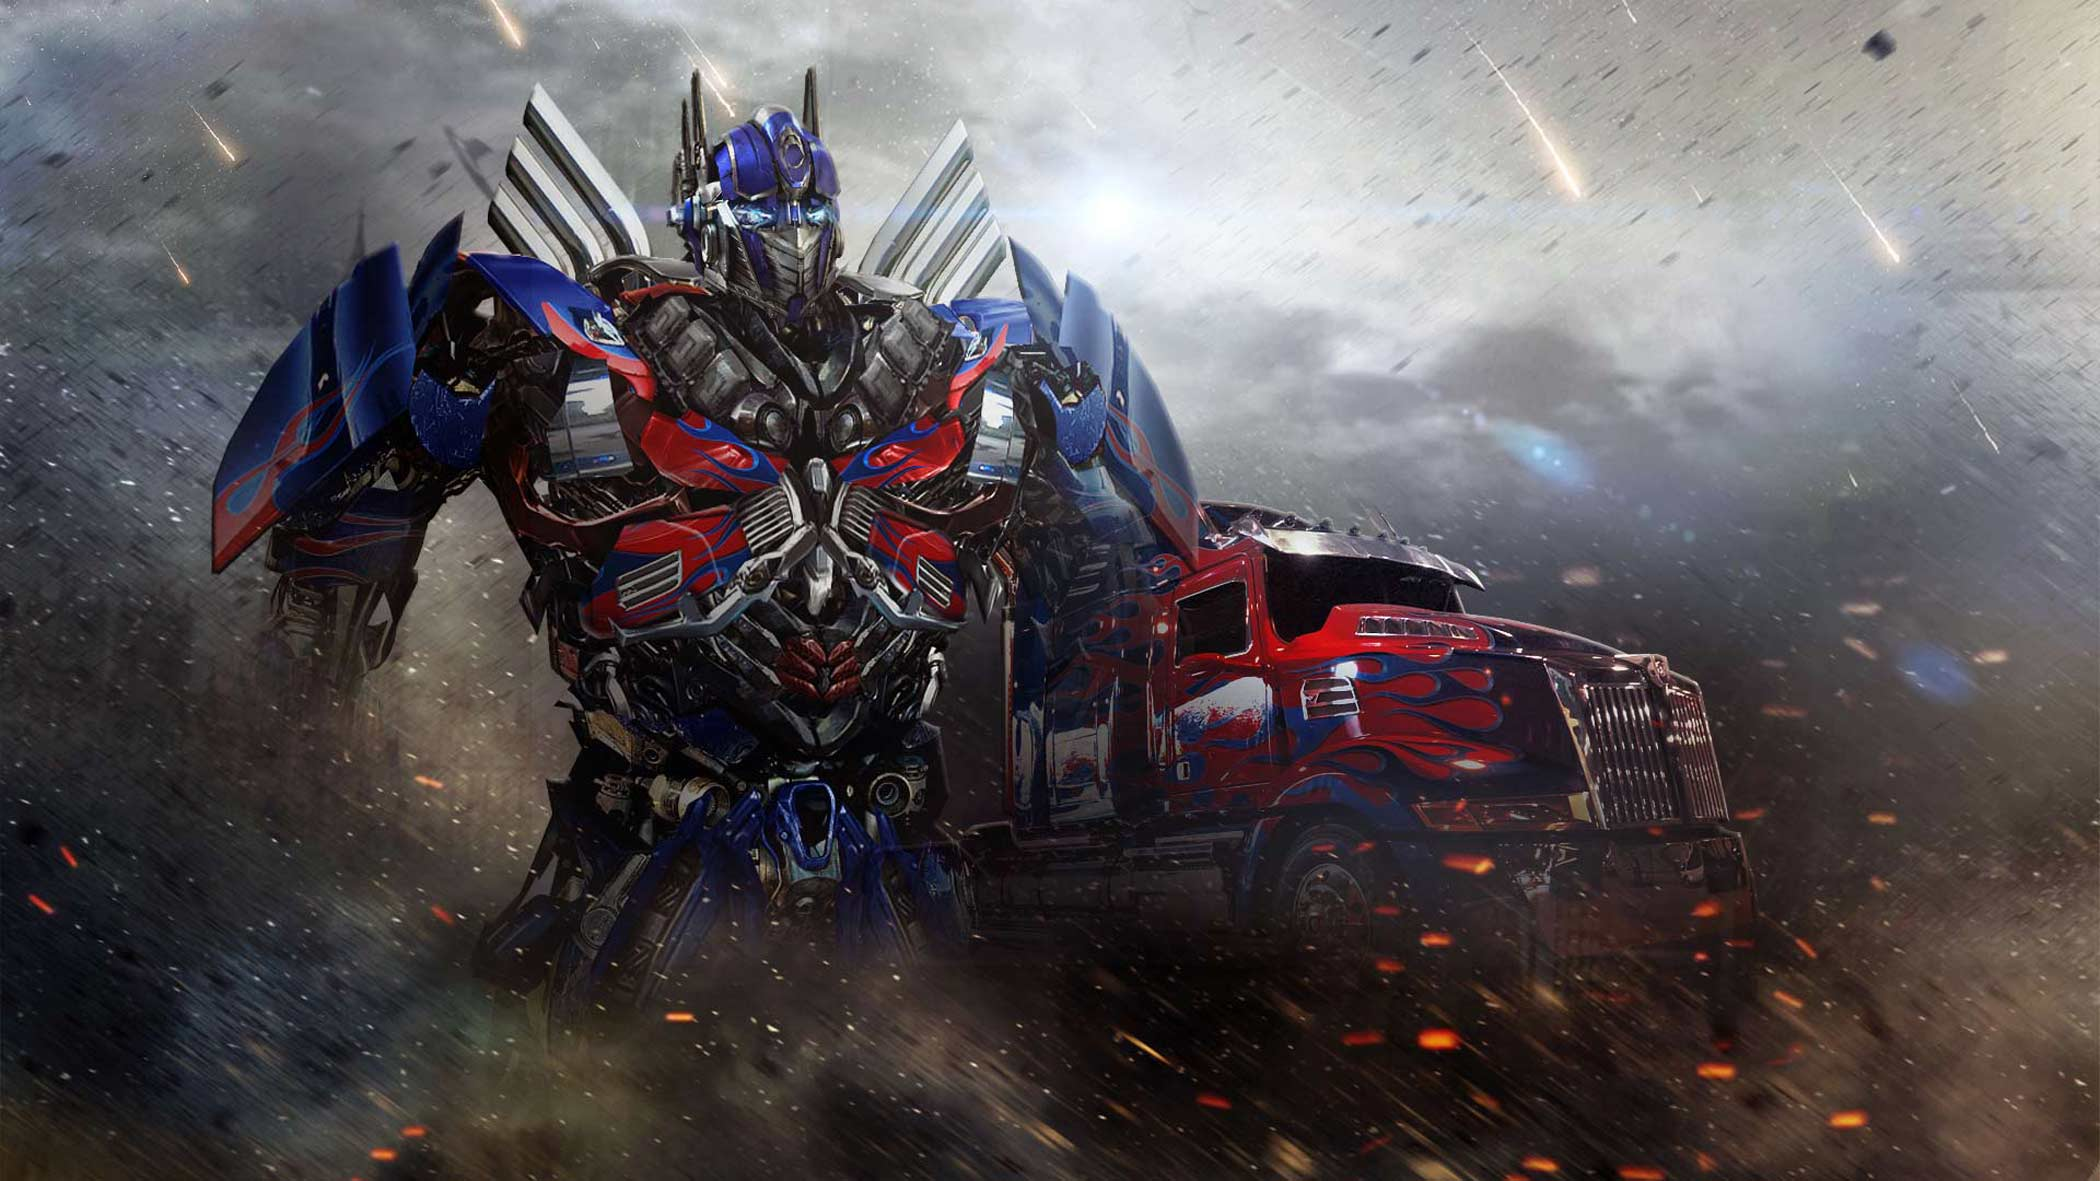
\includegraphics[scale=0.08]{cgi}
            \end{figure}
            \column{0.5\textwidth}
            \begin{figure}
                \centering
                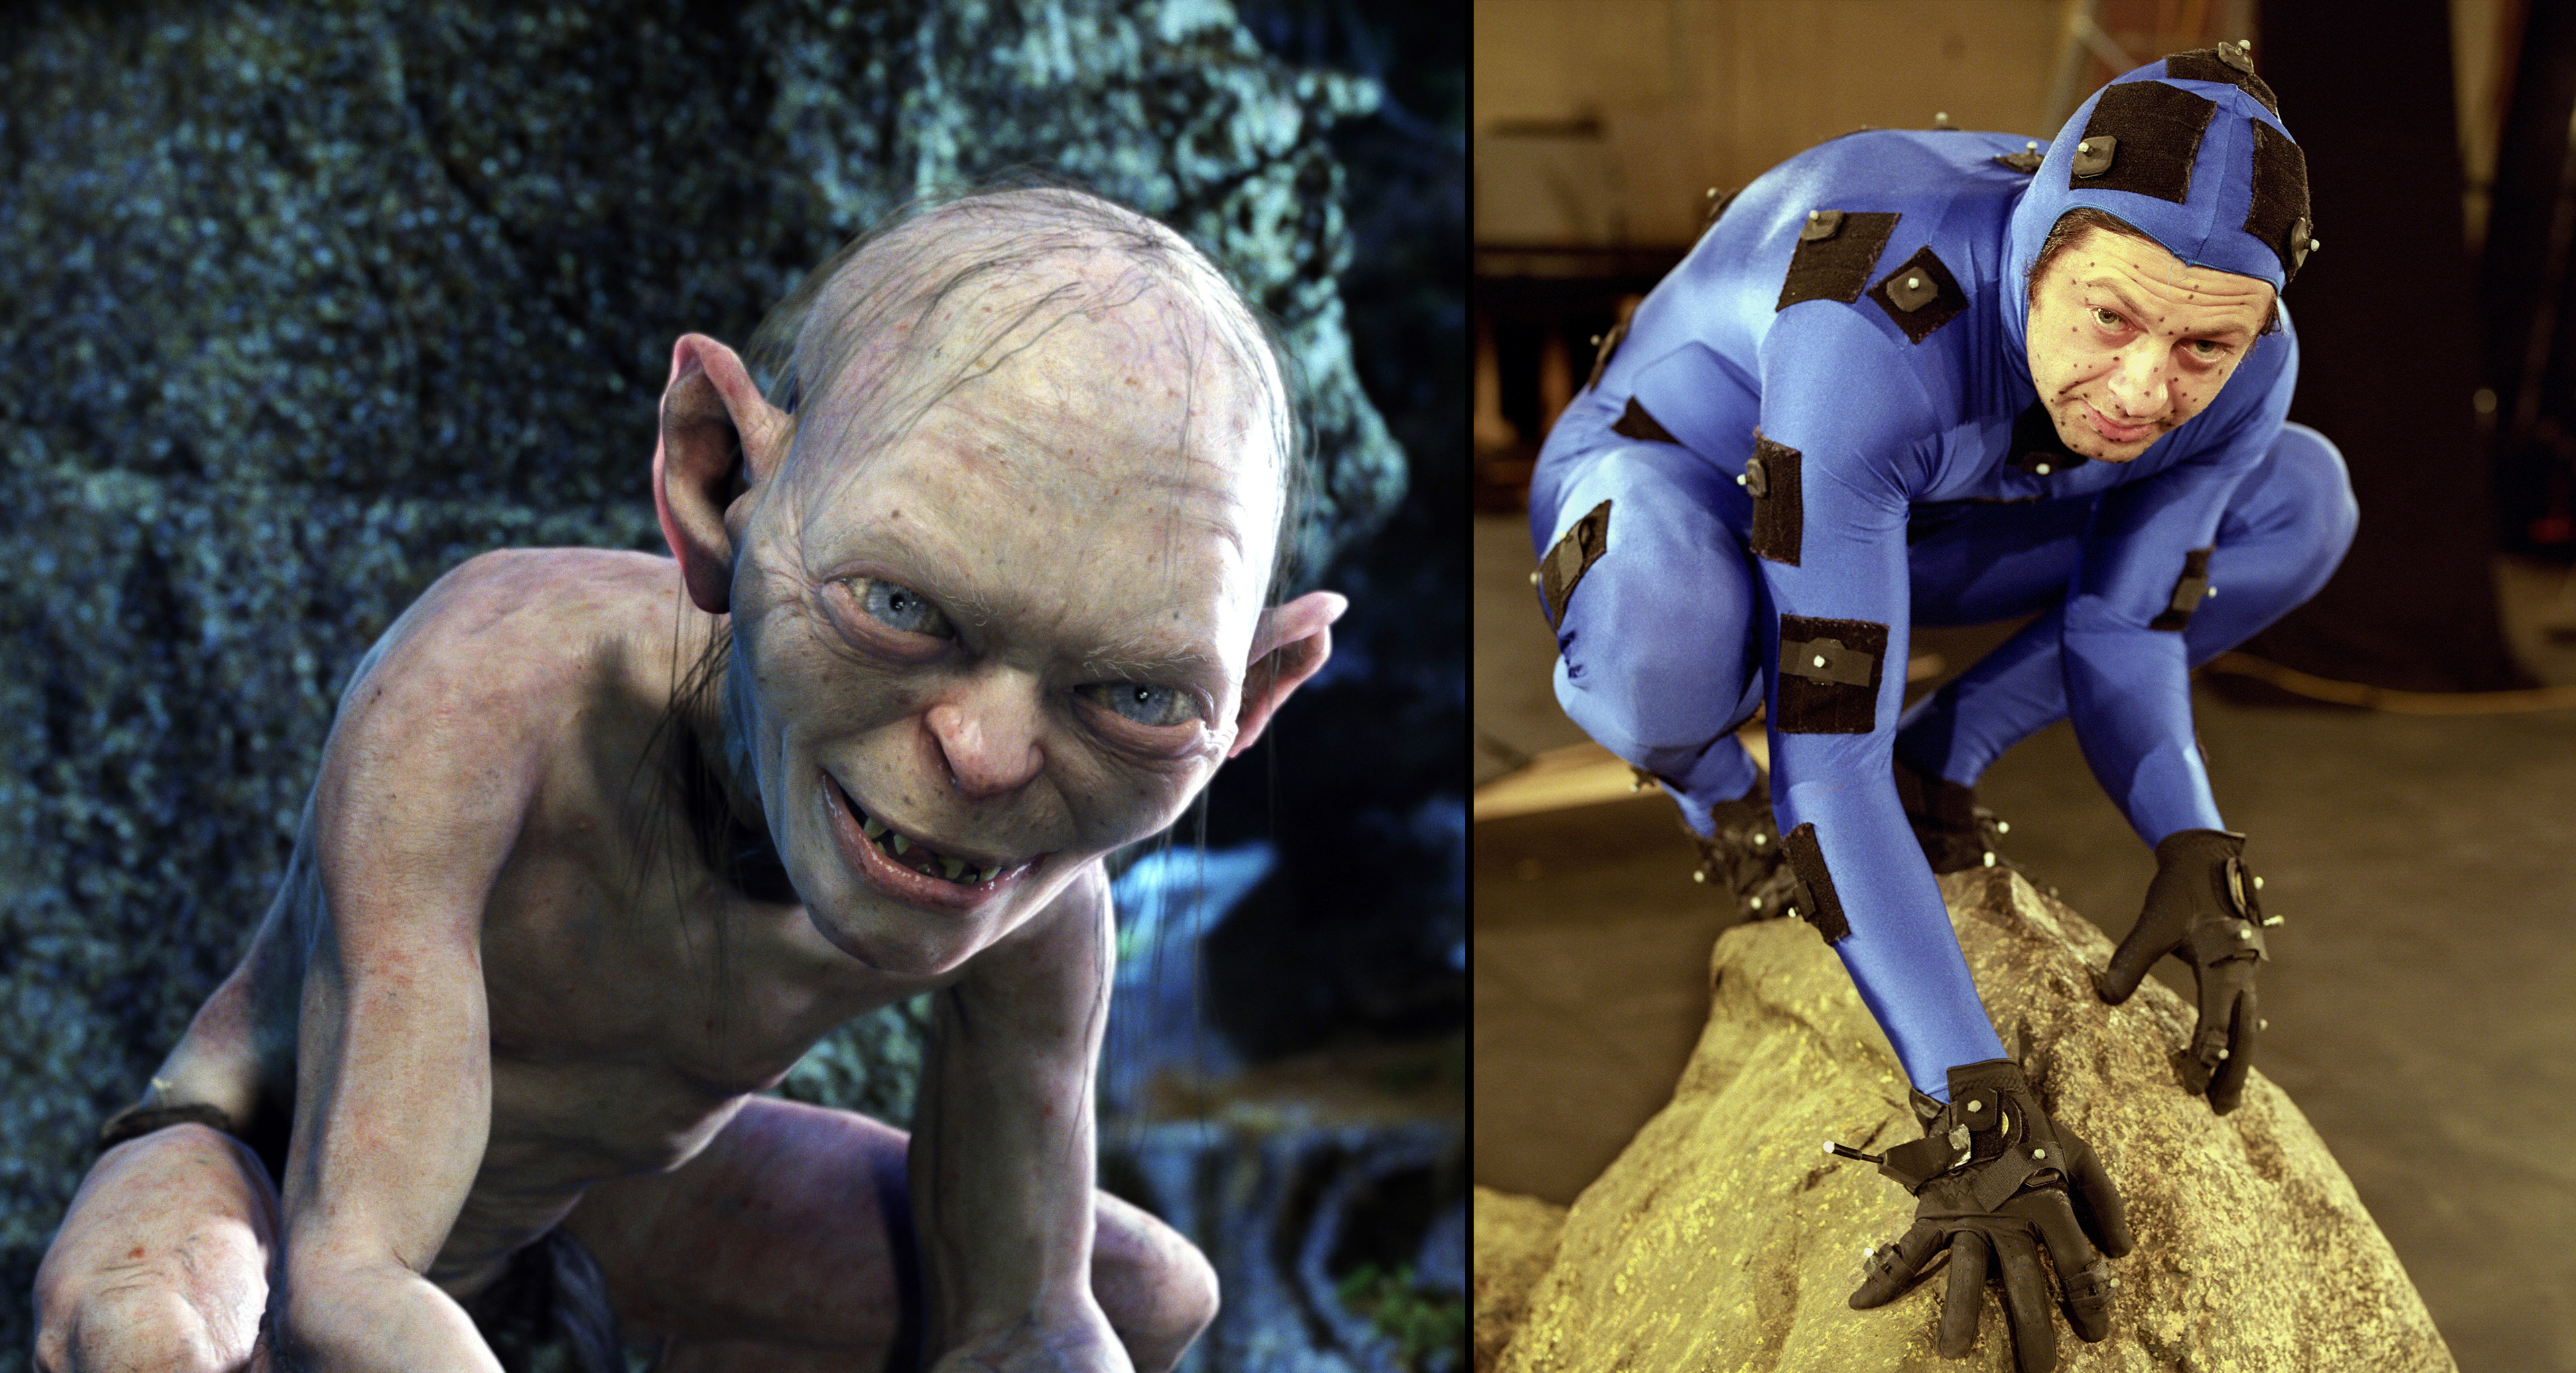
\includegraphics[scale=0.042]{motion_capture}
            \end{figure}
        \end{columns}
    \end{itemize}
\end{frame}

\begin{frame}
    \frametitle{Why Study Programming?}
    \begin{itemize}
        \item Computer Games -- computer graphics, physics
        \begin{columns}
            \column{0.5\textwidth}
            \begin{figure}
                \centering
                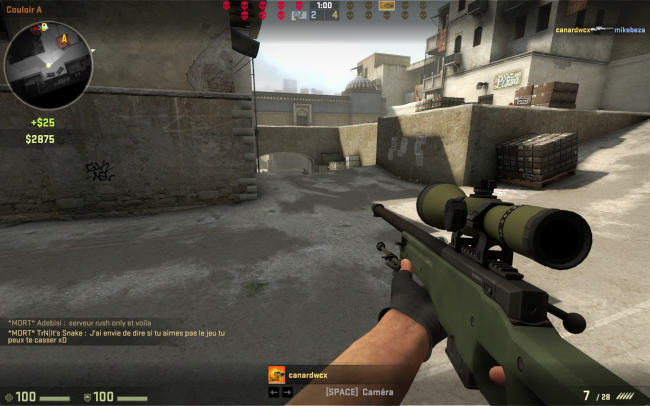
\includegraphics[scale=0.36]{games}
            \end{figure}
            \column{0.5\textwidth}
            \begin{figure}
                \centering
                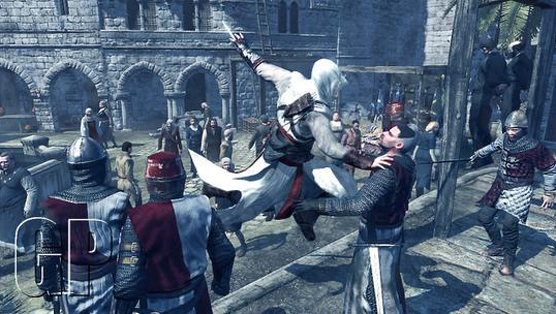
\includegraphics[scale=0.31]{games2}
            \end{figure}
        \end{columns}
    \end{itemize}
\end{frame}

\begin{frame}
    \frametitle{Why Study Programming?}
    \begin{itemize}
        \item Web Development -- website design, information security
        \item Mobile Phones -- mobile applications
        \item Big data Analytics -- data processing, data analysis, machine learning
        \item Banking and Finance -- financial systems simulation, policy modeling
    \end{itemize}
\end{frame}

\begin{frame}
    \frametitle{Evolution of Programming Languages}
    \section{Evolution of Programming Languages} % (fold)
    \label{sec:evolution_of_programming_languages}
    \begin{itemize}
        \item \textbf{Machine Language}
            \begin{itemize}
                \item Lowest-level programming language
                \item 0s and 1s
                \item Easily understood by computers but is almost impossible for humans to use
            \end{itemize}
        \item \textbf{Assembly Language}
            \begin{itemize}
                \item English-like abbreviations such as MOV, ADD etc.
                \item Translated into a machine language by a program called an assembler
                \item Many instructions for even a simple task
            \end{itemize}
        \item \textbf{High level Language}
            \begin{itemize}
                \item Easier to understand for humans
                \item A compiler is required to convert it into machine language
                \item Single statement is enough to carry out many tasks
            \end{itemize}
    \end{itemize}
\end{frame}

\begin{frame}
    \frametitle{Why C++?}
    \section{C++} % (fold)
    \label{sec:why_c}
    \begin{itemize}
        \item \textbf{Why C++?}
            \begin{itemize}
                \item Conciseness
                \item Maintainabilty
                \item Portability
            \end{itemize}
        \item \textbf{Standardization}
            \begin{itemize}
                \item ANSI/ISO standardization
                \item Revisions -- C++ 98, C++ 2003, C++ 2011, C++ 2014
            \end{itemize}
        \item \textbf{C vs. C++}
    \end{itemize}
\end{frame}

\begin{frame}
    \frametitle{C++}
    \begin{itemize}
        \item \textbf{What is Syntax?}
        \item \textbf{What is Algorithm?}
        \item \textbf{What is Code?}
    \end{itemize}
\end{frame}

\begin{frame}
    \frametitle{Criteria for Judging Code Quality}
    \section{Criteria for Judging Code Quality} % (fold)
    \label{sec:criteria_for_judging_code_quality}
    \begin{itemize}
        \item Performance
        \item Simplicity (readability)
        \item Size
        \item Time taken
    \end{itemize}
\end{frame}

\end{document}